\chapter{Design}

%  Software Design

% Typical content will be detailed software design, from architecture to implementation level. As well as your text, you should include UML diagrams, including class structures, activity and sequence diagrams as appropriate. Don't just drop diagrams in willy-nilly, though. Use them strategically to illustrate points in your text. Remember that 'a picture is worth a thousand words' (we don't apply this rule literally) but pictures on their own don't explain everything.

%  Hardware Design

% If your project involves building hardware, give full details about the process here. Include diagrams as appropriate Use them strategically to illustrate points in your text. Remember that 'a picture is worth a thousand words' (we don't apply this rule literally) but pictures on their own don't explain everything. If your project requires electronics and/or mechanical design, don't forget to include that. Photos, CAD drawings, electronic schematics and other diagrams are welcome.

% Experiment design

% If you are going to evaluate your software or hardware by means of any tests or surveys, then explain their design here. If you are doing other experiments (for example measuring the performance of algorithms, extracting data from environmental monitoring systems or evaluating the performance of mechanisms) then you should explain how you have designed the experiments, how they must be conducted and what you expect to learn from them. This is especially important for research-oriented projects.

% Extra

% consider scalability, reliability, efficiency, maintainability, resilience, security, usability and accessibility.

\clearpage
\section{Hardware}

\newpage

\subsection{Development Cards}

In order to build and test the real time software, dedicated development hardware is required to ensure an isolated testing environment.

These test cards consist of a Raspberry Pi Compute Module 4 (CM4).
This contains the same overall hardware as the standard raspberry pi 4.
EMMC flash for high vibration environments.
Exception being the ethernet IC and EMMC flash (This later caused problems with compiling the operating system and bootloader)

Key requirement is remote debugging, full remote power and data control.
Also placed in a rack
Selected the Pi KVM project for remote control as is supports deploy as well as additional GPIO control.

The CM4s display is captured using the CSI port on the KVM with a HDMI to CSI converter.
The power is controlled using a relay, that controls the 12v supply to the CM4.
The signal flags of the EMMC storage are directly connected to the KVM. EXPLAIN the signal flags
These are configured in the KVM user interface
UART is connected to a USB serial converter.
USB host is connected to the KVM for flashing the CM4.
Finally a debugger (JTAG) in case of modifications to the kernel itself.

\begin{figure}[ht]
    \centering
        \begin{tikzpicture}  
            \node[block, text width=1.75cm ] (h) {HDMI\\Capture};  
            \node[block, text width=1.75cm, right=0.1cm of h] (u) {USB\\Serial};  
            \node[block, text width=1.75cm, right=0.1cm of u] (j) {JTAG\\Debugger};  
            \node[block, text width=1.75cm, right=0.1cm of j] (p) {Power\\Relay};

            \node[block, text width=1.75cm, right=0.1cm of p] (m) {Flash\\Mode};
            \node[block, text width=1.75cm, right=0.1cm of m] (l) {Flash\\Lock};
            \node[block, text width=1.75cm, right=0.1cm of l] (f) {USB};

            \node[block, text width=11.75cm, above=1cm of p] (d) {Development Card};  
            \node[block, text width=11.75cm, below=1cm of p] (k) {Remote KVM};  

            \draw[<->,thick] ([xshift=-4.5cm]d.south) to node [midway,fill=white] {HDMI} (h.north);
            \draw[<->,thick] ([xshift=-3cm]d.south) to node [midway,fill=white] {UART} (u.north);
            \draw[<->,thick] ([xshift=-1.5cm]d.south) to node [midway,fill=white] {JTAG} (j.north);
            \draw[<->,thick] ([xshift=-0cm]d.south) to node [midway,fill=white] {12V} (p.north);
            \draw[<->,thick] ([xshift=1.5cm]d.south) edge (m.north);
            \draw[<->,thick] ([xshift=3cm]d.south) edge (l.north);
            \draw[<->,thick] ([xshift=4.5cm]d.south) edge (f.north);

            \draw[<->,thick] (h.south) to node [midway,fill=white] {CSI} ([xshift=-4.5cm]k.north);
            \draw[<->,thick] (u.south) to node [midway,fill=white] {USB} ([xshift=-3cm]k.north);
            \draw[<->,thick] (j.south) to node [midway,fill=white] {USB} ([xshift=-1.5cm]k.north);
            \draw[<->,thick] (p.south) to node [midway,fill=white] {GPIO} ([xshift=0cm]k.north);
            \draw[<->,thick] (m.south) to node [midway,fill=white] {GPIO} ([xshift=1.5cm]k.north);
            \draw[<->,thick] (l.south) to node [midway,fill=white] {GPIO} ([xshift=3cm]k.north);
            \draw[<->,thick] (f.south) to node [midway,fill=white] {USB} ([xshift=4.5cm]k.north);
        \end{tikzpicture}  
    \caption[Development Hardware]
    {Development Hardware}
    \label{fig:developmentHardware}
\end{figure}


Two of these so that multiple benchmarking activities can be performed at once and compared.


Use the uBoot boot loader.
This allows the development images to be loaded over TFTP, we have a dedicated tftp boot server.

Connected to a managed switch. The test harness is connected to this on a separate VLAN.

% \begin{figure}
%     \centering
%     \resizebox{\columnwidth}{!}{
%         %
%         \begin{tikzpicture}  
%             \node[block] (d1) {Development Card};  
%             \node[block,right=of a] (k1) {Debug KVM};

%             \node[block,below=of a] (d) {Reciever};  
%             \node[block,right=of d] (e) {Destination};  

%             % \node[draw,inner xsep=4mm,inner ysep=7mm,fit=(a)(b) ] (c1) {Application Layer};
%             % \node[draw,inner xsep=4mm,inner ysep=7mm,fit=(d)(e) ] {Infrastructure Layer};  
%             % \node[draw,inner xsep=4mm,inner ysep=7mm,fit=(d)(e),label={Hardware Layer}]{};
%         \end{tikzpicture}  
%         %
%     }
%     \caption[Heatmap for class distribution in dataset]
%     {Heatmap for class distribution in dataset}
%     \label{fig:heatmap}
% \end{figure}

\begin{tikzpicture}[node distance=1.75cm]
    \node[draw] (node1) {Node 1};
    \node[draw, below of=node1] (node2) {Node 2};
    
    % Create a node that fits both node1 and node2
    \node[fit=(node1)(node2), draw, inner sep=0pt] (fitnode) {};
    
    % Adjusting the fitting node to match the sizes
    \node[above right] at (fitnode.south west) {Fitting Node};
\end{tikzpicture}

\begin{tikzpicture}[
    mymatrix/.style={matrix of nodes, nodes=block, row sep=1em},
    mycontainer/.style={draw=gray, inner sep=1ex},
    typetag/.style={draw=gray, inner sep=1ex, anchor=west},
    title/.style={draw=none, color=gray, inner sep=0pt}
    ]
    \matrix[mymatrix] (mx1) {
      |[title]|Decomposition \\
      Independent \\
      Reduction \\
      DivideAndConquer \\
    };
    \matrix[mymatrix, right=of mx1.north east, matrix anchor=north west] (mx2) {
      |[title]|Dependency \\
      Atomic \\
      Range \\
    };
    \node[mycontainer, fit=(mx1)] {};
    \node[mycontainer, fit=(mx2)] {};
  
  \end{tikzpicture}

\clearpage
\graphicspath{{main/design/hardware/graphics/}}

\subsection{Development Test Harness} \label{sec:testHarness}

Similar to the development cards, dedicated and isolated hardware was required for the test harness. This was to perform validation against the developed software to ensure the real-time requirements were maintained. Through the harness, an example control loop implementation could be simulated to ensure all deadlines are met during a live software update.

\begin{figure}[ht]
    \centering
    \begin{tikzpicture}  
        \node[block] (gen) {Signal\\Generator}; 
        \node[block, right=2cm of gen] (sw) {Software\\Infrastructure};
        \node[block, right=2cm of sw] (rcv) {Signal\\Receiver};  
        
        \node[block, text width=12cm, minimum height=1cm, below=1cm of sw] (har) {Harness}; 
        \node[block, minimum height=1cm, below=1cm of har] (ana) {Analyser};  

        \draw[->,thick] (gen) edge (sw);
        \draw[->,thick] (sw) edge (rcv);

        \draw[->,thick] (gen.south) edge ([xshift=-5.3cm]har.north);
        \draw[->,thick] (rcv.south) edge ([xshift=5.3cm]har.north);

        \draw[->,thick] (har) edge (ana);
    \end{tikzpicture}  
    \caption[Test harness design]
    {Test harness design}
    \label{fig:testHarnessDesign}
\end{figure}

% WRONG TENSE
\autoref{fig:testHarnessDesign} contains a signal generator, this randomly produces a signal and outputs a packet. These packets are ingested by the software infrastructure where processing occurs. An output packet is subsequently generated (mirroring the input) and sent to a signal receiver, which captures this packet.

The signal generator and receiver output their current state over discrete digital signals so that a logic analyser can record the state of the system over time. Specifically the states can be compared to measure the complete system latency during standard operation and software update. If the generator and receiver produce additional reference clock signals, the logic analyser can more closely calculate the software infrastructure induced latency.

The theoretical logic analyser output is displayed in \autoref{fig:testHarnessCapture}. The latency between generate and receive is shown on the latency channel.

\begin{figure}[ht]
    \centering
    \begin{tikztimingtable}[%
        timing/dslope=0.1,
        timing/.style={x=2ex,y=2ex},
        x=2ex,
        timing/rowdist=3ex,
    ]
        \busref{Generator Clock} & 2l 10{4c} \\
        \busref{Reciever Clock } & 11{4c} \\
        \busref{Generator Signal} & 6h 16l 16h 4l \\
        \busref{Reciever Signal} & 8h 16l 16h 4l \\

        \busref{Latency} & 6l D{} 14l  D{} 14l D{} 2l \\
        \extracode
            \begin{pgfonlayer}{background}
            \begin{scope}[semitransparent ,semithick]
                \vertlines[darkgray,dotted]{0.5,1.0 ,...,20.0}
            \end{scope}
        \end{pgfonlayer}
    \end{tikztimingtable}
    \caption[Test harness capture]
    {Test harness capture}
    \label{fig:testHarnessCapture}
\end{figure}

The generator, receiver and logic analyser were all implemented using the RP2040 microprocessor from Raspberry Pi for hardware simplification. The two controllers that performed message communication used the W5500 chip to send UDP packets over ethernet, this integrated nicely with software infrastructure. The co-processor offloads the complex ethernet drivers and communicates to the main processor over SPI. The embedded network switch selected to connect the different elements of the test harness with the development cards was the SwitchBlox 'Small Ethernet Switch'.

\autoref{fig:TestHardwareFrameMount} displays the frame mount designed in Fusion 360 and 3D printed, to hold the components together in a single package. Harness is shown assembled in \autoref{fig:TestHarnessHardware}.

\begin{figure}[ht]
    \centering
    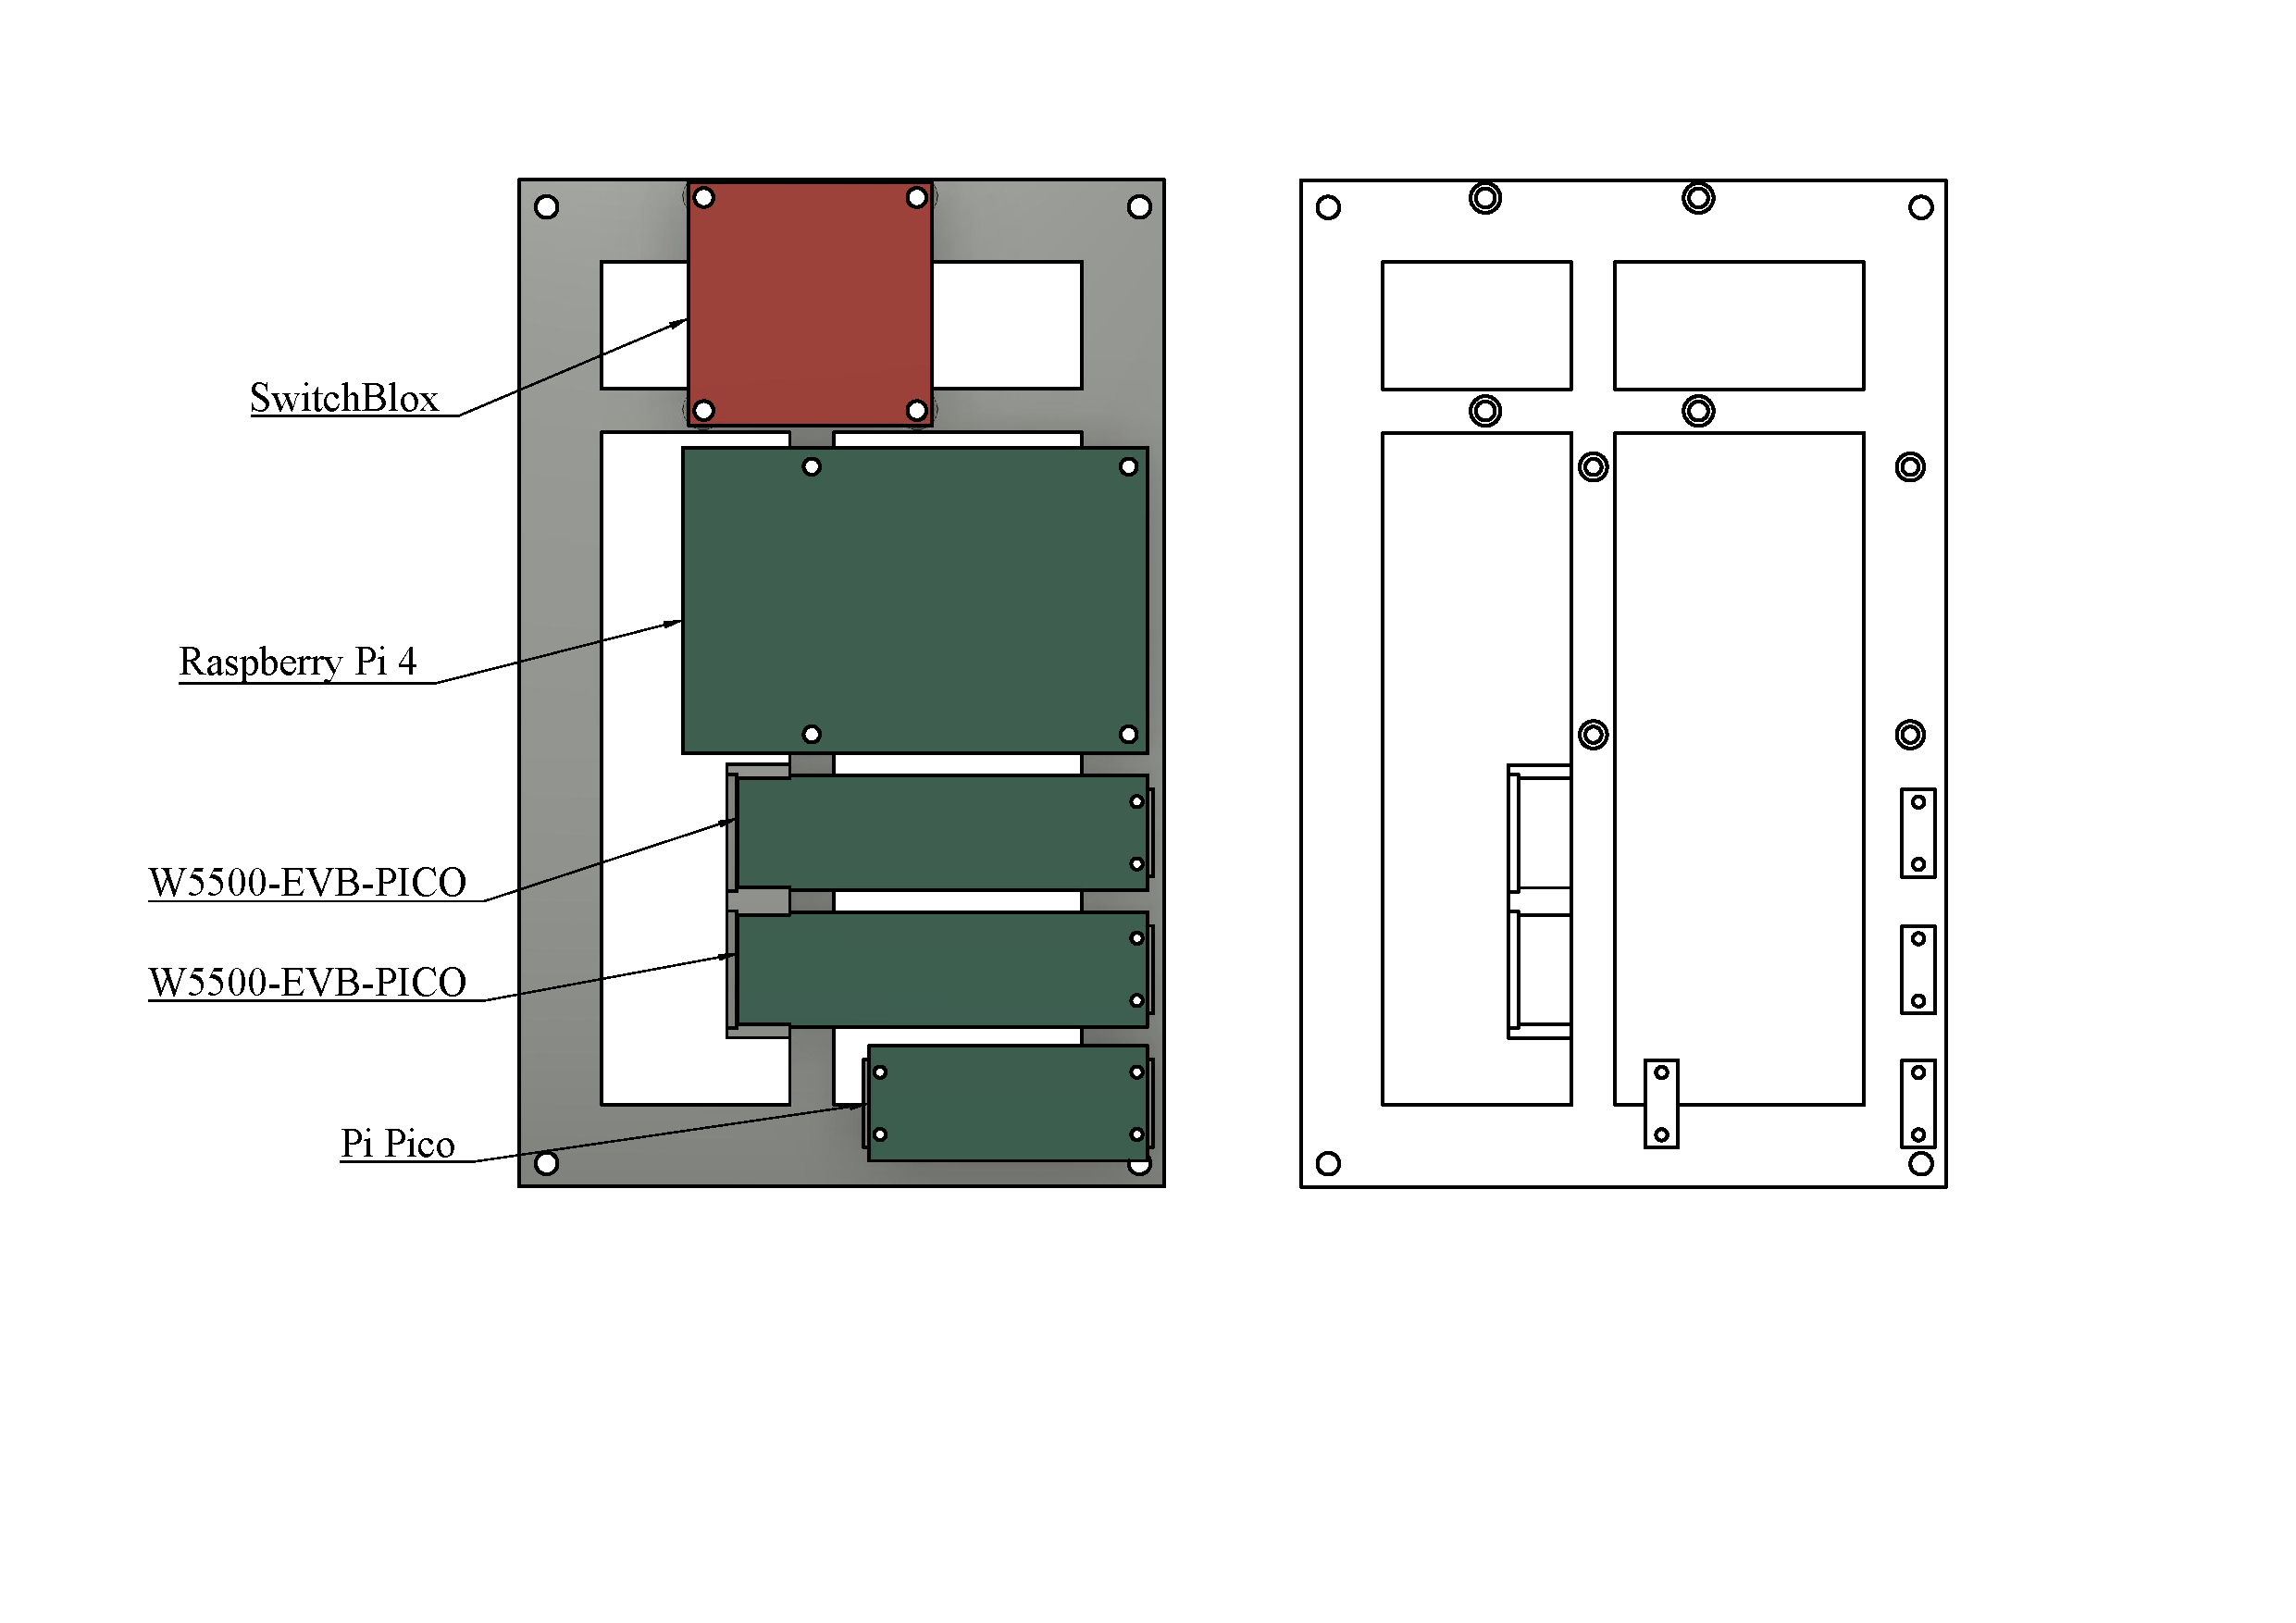
\includegraphics[width=\textwidth, clip, trim=0.5cm 7cm 0.5cm 2cm]{TestHardwareFrameMount.pdf}
    \caption[Test harness hardware frame mount design]
    {Test harness hardware frame mount design}
    \label{fig:TestHardwareFrameMount}
\end{figure}

\begin{figure}[ht]
    \centering
    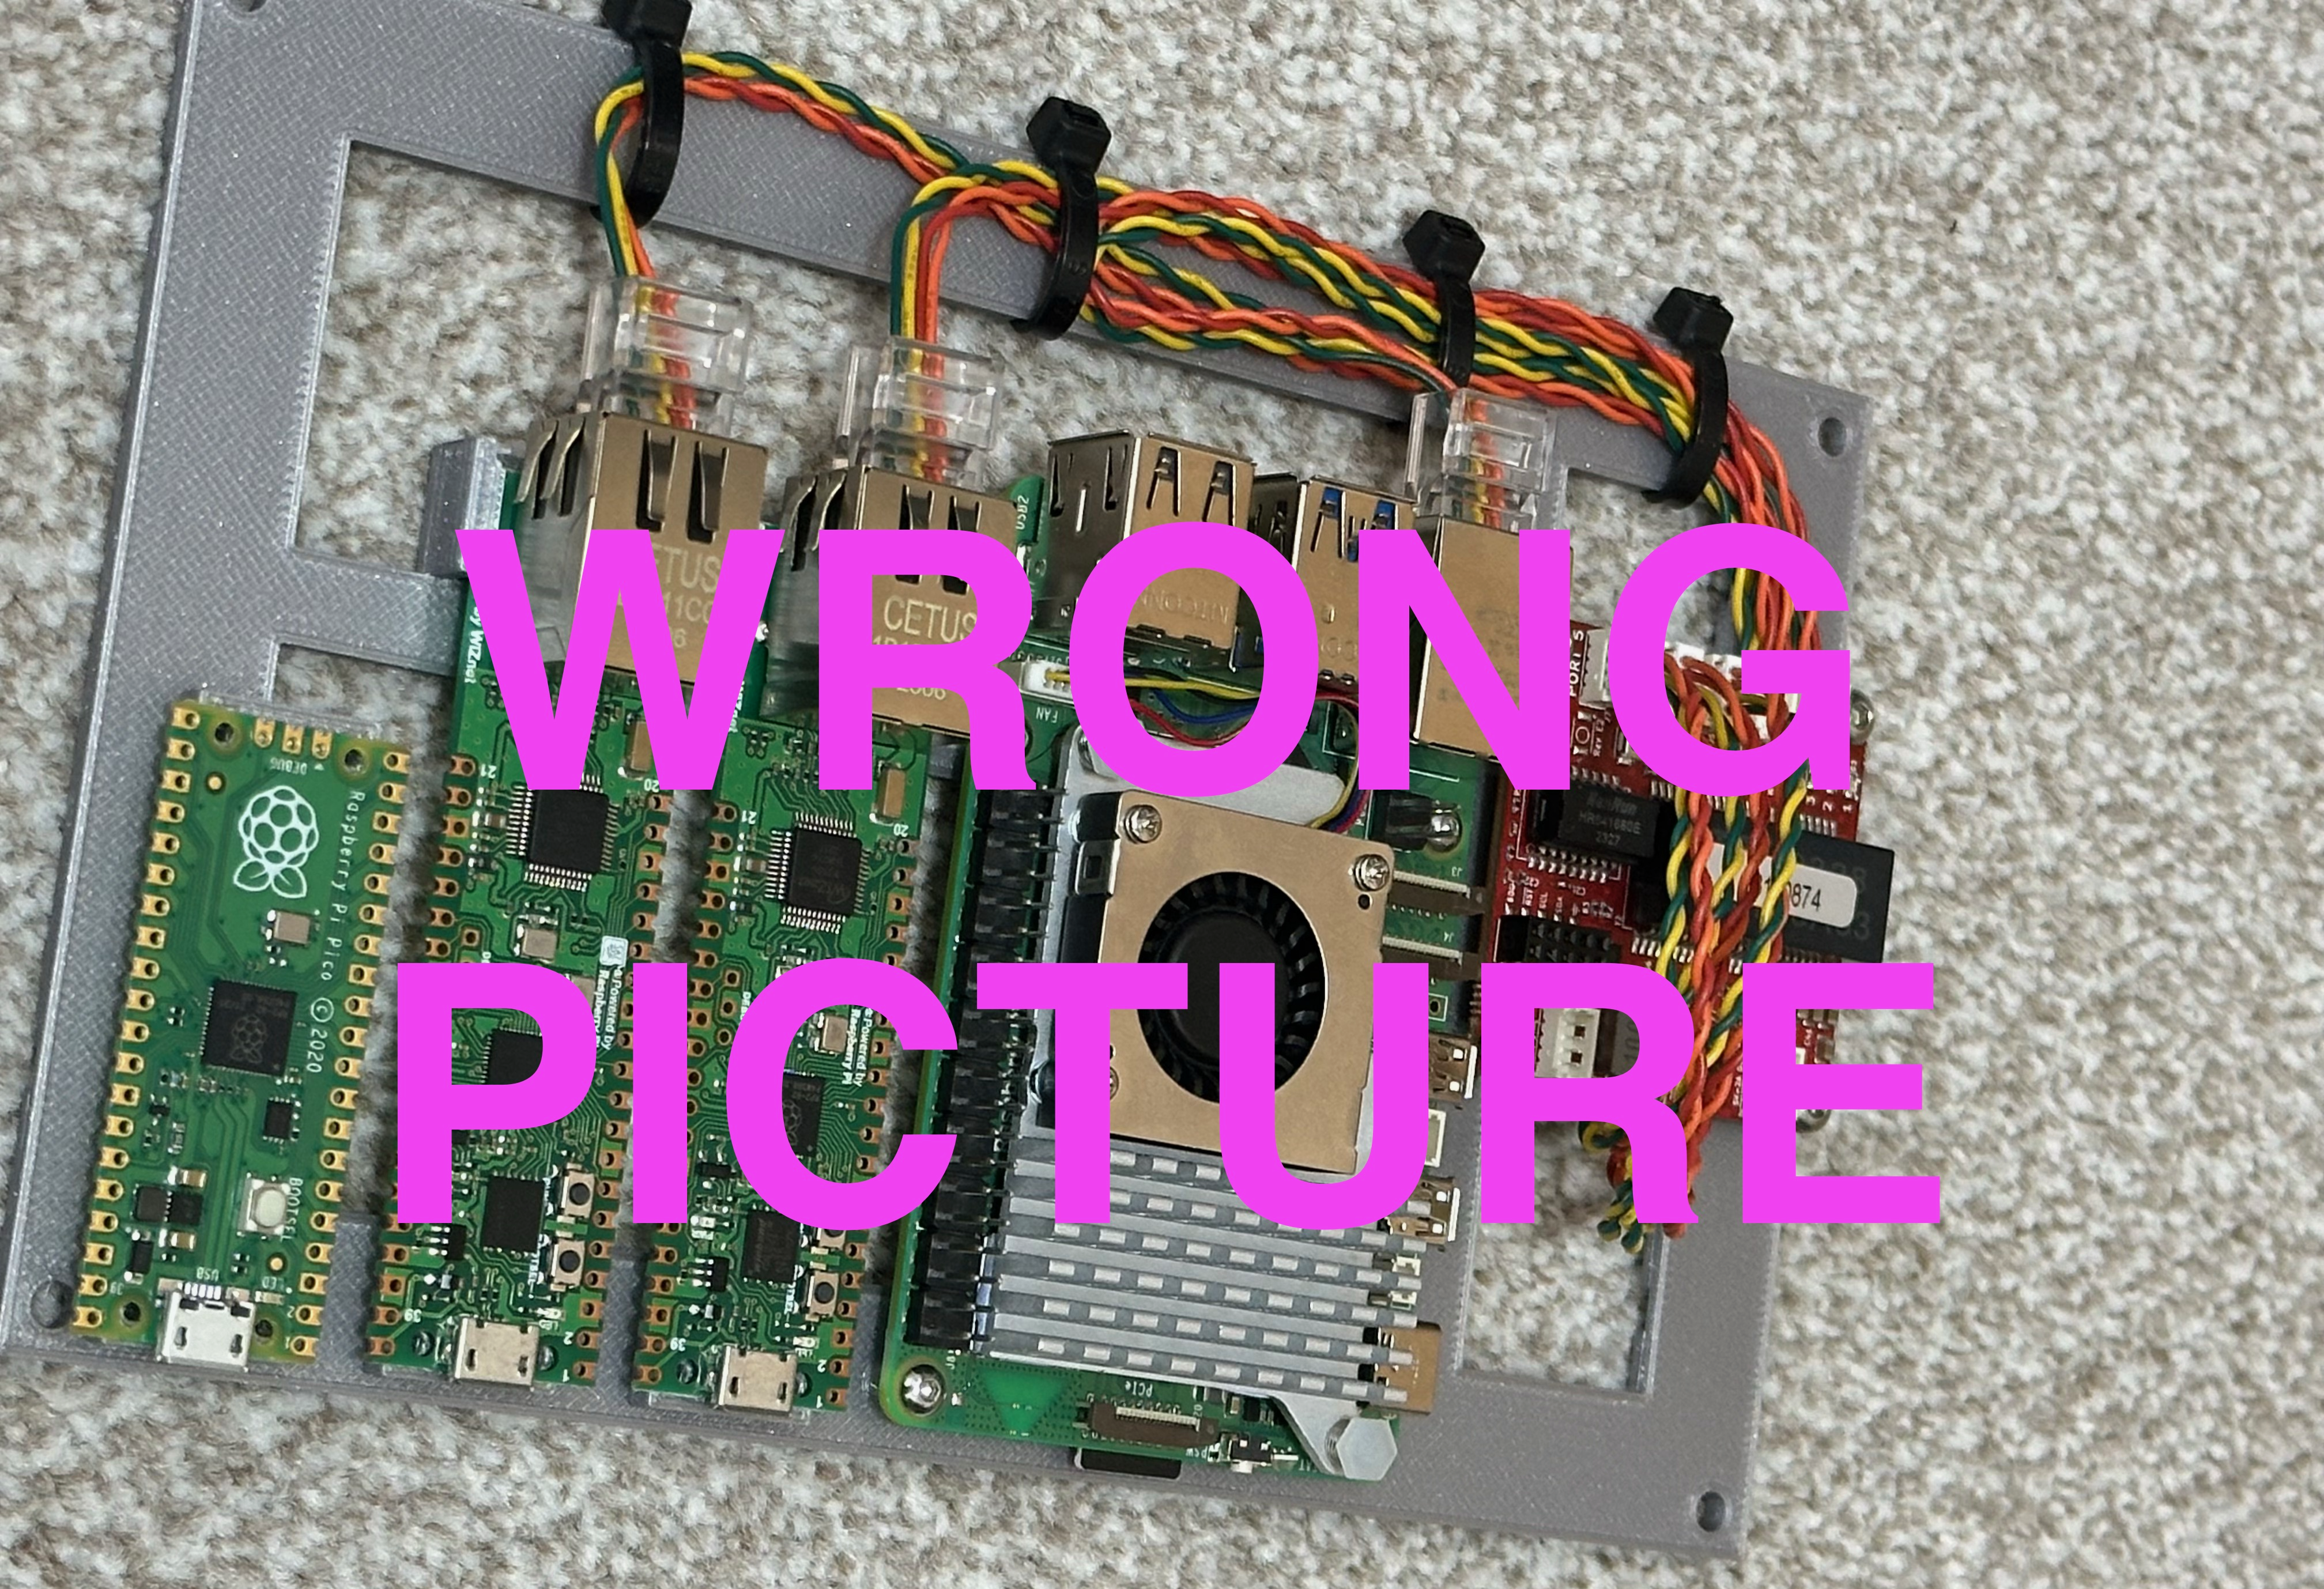
\includegraphics[width=10cm, clip]{TestHarnessHardware}
    \caption[Test harness hardware assembled]
    {Test harness hardware assembled}
    \label{fig:TestHarnessHardware}
\end{figure}

\clearpage


\begin{table}[ht]
    \centering
    \begin{tabular}{ c|ccc } 
        \hline
        Name & Manufacturer & Quantity & Task \\ 
        \hline
        \href{https://www.raspberrypi.com/products/raspberry-pi-4-model-b/}{Raspberry Pi 4} & Raspberry Pi & 1 & Boot Server \\ 
        \href{https://www.raspberrypi.com/products/raspberry-pi-pico/}{Raspberry Pi Pico} & Raspberry Pi & 3 & Test Hardware \\ 
        \href{https://botblox.io/products/small-ethernet-switch}{Small Ethernet Switch} & SwitchBlox & 1 & Network Switch \\ 
    \end{tabular}
    \caption[Development hardware bill-of-materials]
    {Development hardware bill-of-materials}
    \label{tbl:TestHarnessHardwareBOM}
\end{table}



The chosen logic analyser software was PulseView as it is open-source and supports many different logic analyser devices \autocite{pulseviewPulseViewSigrok}. Boards which use the RP2040 microprocessor (Pi Pico) can use the ULA logic analyser firmware \autocite{domnikovDotcypressUla2024}.

When flashed, the Pi Pico can capture the status of 16 input channels at specified frequencies. An example capture is shown in \autoref{fig:testHarnessPluseViewCapture}.

\begin{figure}[ht]
    \centering
    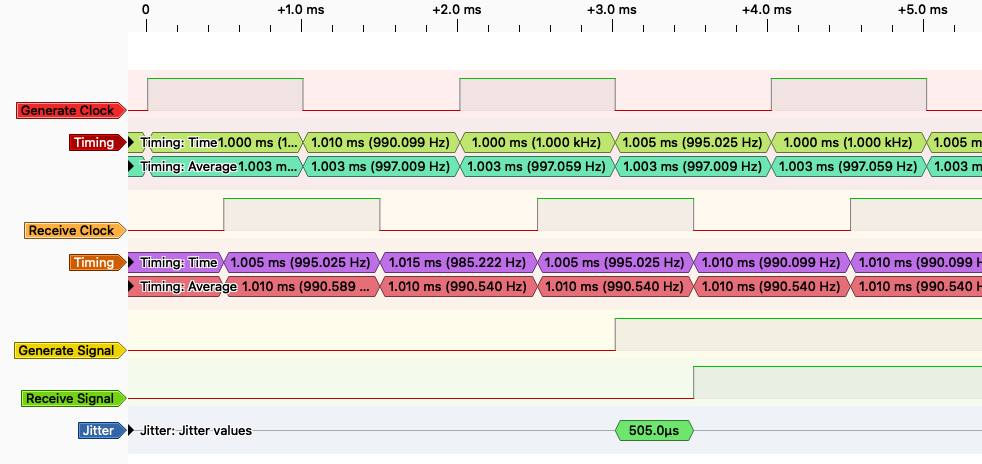
\includegraphics[width=\textwidth]{testHarnessPluseViewCapture.png}
    \caption[Test harness PluseView capture]
    {Test harness PluseView capture}
    \label{fig:testHarnessPluseViewCapture}
\end{figure}


\clearpage
\clearpage
\section{Runtime}
\clearpage
\graphicspath{{main/design/software/graphics/}}

\subsection{Operating Systems} \label{sec:operatingSystems}

\textcite{serinoSurveyRealTimeOperating2019} compiled a comparison of the differences between 
\textcolor{red}{NOT DONE!}

VxWorks, RTLinux and FreeRTOS. 

RTLinux - General perpous 

VxWorks - commerical hard real time operating system

FreeRTOS - open source hard real time


Alternatively the PREEMPT\_RT patch is available for mainline Linux, that aims to minimise the amount of kernel code that is non-preemptible  \autocite{RealtimeDocumentationStart}. The patch prefers deterministic behaviour over throughout and makes a number of changes to the kernel including replacing kernel locks with rtmutexes. However some resource management functions (memory management) have indeterminate maximum latencies. This patch results in a soft real-time operating system as the kernel is not designed to guarantee deadlines. \autocite{maddenChallengesUsingLinux2019}

Although Linux with the RT patch was not strictly suitable for real-time applications it was chosen as the operating system for developing the software infrastructure. This was because Linux has a wide support for software libraries, build environments and has many user guides for development.
Linux also supports containerization through cgroups and namespaces, which could be useful for creating the isolated processing environments \autocite{huynhKubernetesStoryLinux2023}. In case of a real deployment, the software should use a more suitable operating system such as VxWorks. Both OS's are Unix-like so should porting the software should be fairly trivial.

% If required real-time not certified a certified operating system

\subsection{Hypervisors}

\textcolor{red}{NOT DONE!!}

Why xen? 

This is because KVM is implemented on top of the Linux kernel.

To reap the benefits of dynamic updates it is preferred that the hypervisor is independent of the operating system (explain why).
Also, in a true real-time system it is unusual to use linux. Rather a more preferable OS such as Zephyr or FreeRTOS (Free and open source solutions used.)


\autocite{ayresVirtualisationMeansDynamic2019} completed a short study into the different available virtualisation technologies for embedded safety critical systems.

VxWorks, Jailhouse, KVM, Xen, Sel 4
All have public support for the raspberry pi 4

Xen was selected for te hypervisor for its independence from linux and open source nature



HVM, PV, PVH
Xen uses para-virtualization and a modified version of the Linux kernel can run as a guest OS.

EXPLAIN RT LINUX

% why xen for ramdisk etc
% virtual switch, arrangement of dom0 with hardware control

\subsection{Build Process}

\textcolor{red}{NOT DONE!!!}

All software images for the development cards were created using the Yocto Project build environment because of it's support for both Linux and Xen. Although some images for Linux were initially created manually, this process was exceptionally slow and an inefficient use of time.

Yocto is an open source project that uses various layers to build an image using scripts.

\begin{itemize}
    \item poky
    \item meta-openembedded
    \item meta-raspberrypi
    \item meta-virtualization
\end{itemize}

\begin{itemize}
    \item meta-cm4-uboot-fix
    \item meta-rpi4-kernel
\end{itemize}

xen version 

linux version

uboot version

Use the uBoot boot loader.
\clearpage
\graphicspath{{main/design/runtime/graphics/}}

\subsection{Analysis}

To select the most optimal environment to develop the software infrastructure upon, a series of benchmarking activities were carried out. These focused on evaluating the operating systems and hypervisors which could operate in a real-time environment. Comparing bare-metal Linux and Xen with Linux VMs should give a good method to estimate the specific latencies brough about by Xen.

\subsubsection{Test Suite}
There are several tools that can be used to analyse the real-time performance of an operating system. RT-Tests is a test suite that contains programs to test the various real-time Linux features.

The RT-Tests suite includes a cyclictest program. This is a simple yet effective program that can be used to estimate the real-time latencies in a system. It measures real-time jitter by creating a interrupt event at a specific time in the future and measuring the time delay between the requested wake-up and actual wake-up time. While this provides a good method for identifying operating system induced latency and jitter it does not isolate latencies induced by hardware or low-level firmware. At this stage it can be assumed that the selected development targets do not induce significant latencies.

% Stress-ng
Another tool that can be used during real-time testing is stress-ng (stress next generation) from \textcite{kingColinIanKingStressng2024}. This program can put artificial loads onto a Linux system. While sustained memory and CPU pressures are unlikely in a real application scenario it is important to ensure that the real-time characteristics of an OS do not significantly change.

\clearpage

\subsubsection{Previous Work}

% The paper results
\textcite{abeniUsingXenKVM2020} compiled a similar study into the real-time performance of open source hypervisors. Every hypervisor introduces some latencies into a virtual machine that can affect the correctness of the existing real-time analysis. They compared the performance of both KVM and Xen on various intel x86 processors.

The study found that the KVM hypervisor would be suitable for serving real-time workloads with worst-case latencies under $100\mu$s. This is applicable only when using RT kernels on both the guest and host. Likewise when using the Xen hypervisor the RT kernels on both the guest and host must also be used. Para-virtualised (PV) guests performed well but fully virtualised (HVM) guests did not, under $100\mu$s versus $1000000\mu$s.

% How it applies and differs from our tests
For the purpose of this project the real-time performance on an Arm64 target, the chosen development target, must be specifically analysed. It was reasonable to expect that the performance characteristics may be different between Arm64 and x86 due to the implementation of virtualisation extensions.

\clearpage

\subsubsection{Linux}

To set a baseline the real-time behaviour of Linux with the standard PREEMPT kernel was tested with different artificial loads in the system. Each test ran for exactly 1 hour collecting latency information at an interval of $100{\mu}s$.

Figure \autoref{fig:linux-i100-1h-allcores} displays that when not under load, the standard Linux kernel performs well in a real-time environment. However as soon as load was introduced into the system \autoref{fig:linux-i100-1h-allcores-sc4} and \autoref{fig:linux-i100-1h-allcores-sm4} the real-time performance was significantly worse.

\begin{figure}[ht]
    \centering
    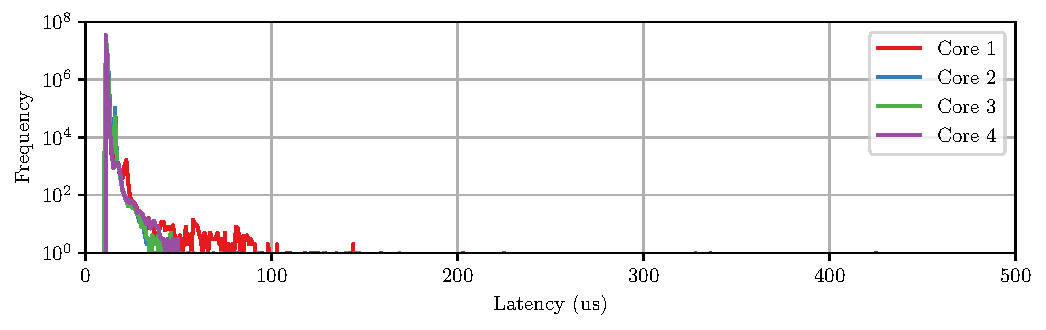
\includegraphics[width=\textwidth]{linux-i100-1h-allcores.pdf}
    \caption[Linux PREEMPT i100 cyclictest results (idle)]
    {Linux PREEMPT i100 cyclictest results (idle)}
    \label{fig:linux-i100-1h-allcores}

    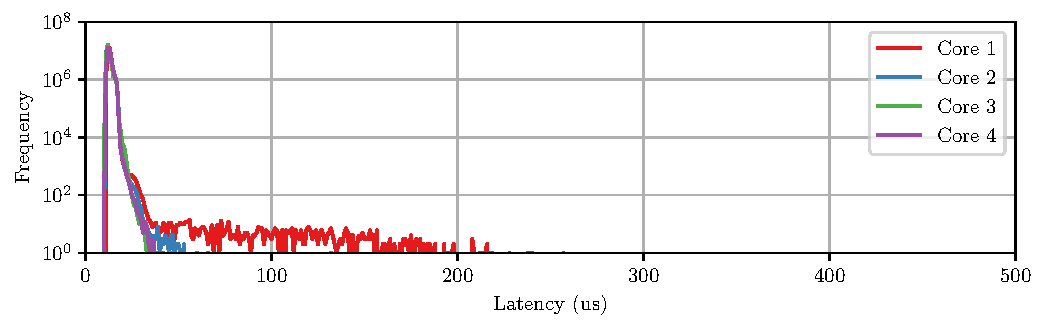
\includegraphics[width=\textwidth]{linux-i100-1h-allcores-sc4.pdf}
    \caption[Linux PREEMPT i100 cyclictest results (cpu load)]
    {Linux PREEMPT i100 cyclictest results (CPU load)}
    \label{fig:linux-i100-1h-allcores-sc4}

    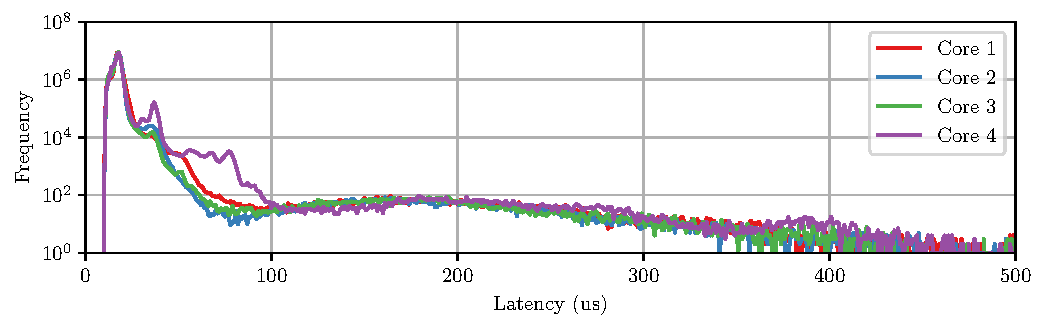
\includegraphics[width=\textwidth]{linux-i100-1h-allcores-sm4.pdf}
    \caption[Linux PREEMPT i100 cyclictest results (memory load)]
    {Linux PREEMPT i100 cyclictest results (memory load)}
    \label{fig:linux-i100-1h-allcores-sm4}
\end{figure}

\clearpage

The following tests in \autoref{fig:linux-rt-i100-1h-allcores}, \autoref{fig:linux-i100-1h-allcores-sc4} and \autoref{fig:linux-rt-i100-1h-allcores-sm4} all used the PREEMPT\_RT kernel. With the same test parameters the system maintained a good response latency even when under load.

\begin{figure}[ht]
    \centering
    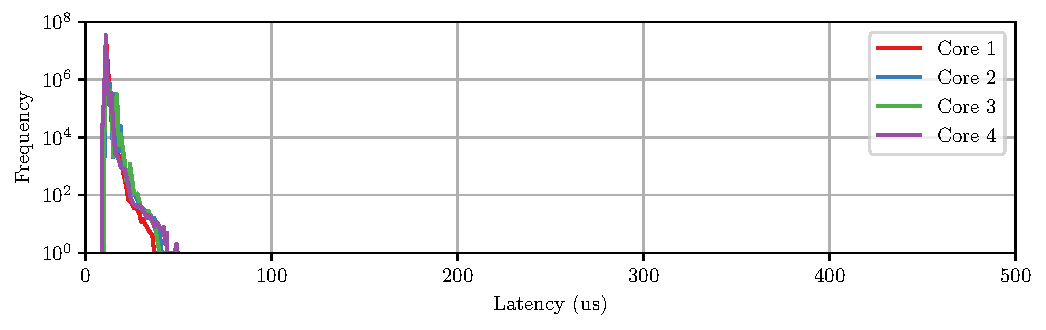
\includegraphics[width=\textwidth]{linux-rt-i100-1h-allcores.pdf}
    \caption[Linux PREEMPT\_RT i100 cyclictest results (idle)]
    {Linux PREEMPT\_RT i100 cyclictest results (idle)}
    \label{fig:linux-rt-i100-1h-allcores}

    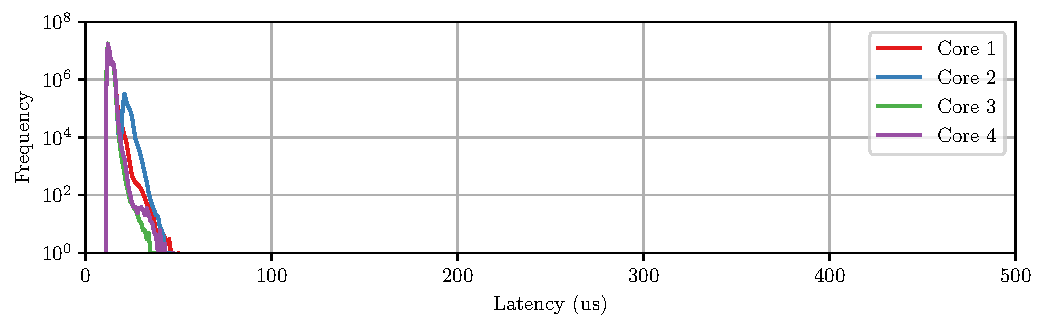
\includegraphics[width=\textwidth]{linux-rt-i100-1h-allcores-sc4.pdf}
    \caption[Linux PREEMPT\_RT i100 cyclictest results (cpu load)]
    {Linux PREEMPT\_RT i100 cyclictest results (cpu load)}
    \label{fig:linux-rt-i100-1h-allcores-sc4}

    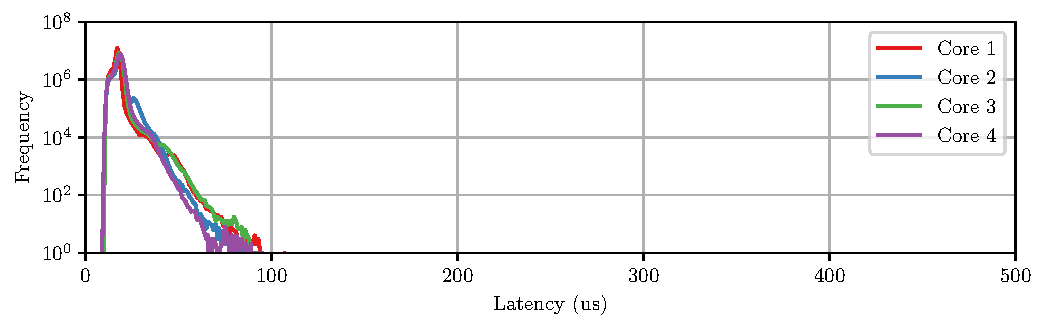
\includegraphics[width=\textwidth]{linux-rt-i100-1h-allcores-sm4.pdf}
    \caption[Linux PREEMPT\_RT i100 cyclictest results (memory load)]
    {Linux PREEMPT\_RT i100 cyclictest results (memory load)}
    \label{fig:linux-rt-i100-1h-allcores-sm4}
\end{figure}

\clearpage

\textbf{Evaluation}

The comparison between both kernels is shown in \autoref{fig:linux-vs-rt-linux-i100-1h-sc4} and \autoref{fig:linux-vs-rt-linux-i100-1h-sm4} displays that the real-time kernel patch works as expected.

Memory tests particularly strained the memory resources allocation processes of the kernel and affected the real time performance more than CPU load. This is because many parts of the Linux kernel resource allocation have indeterminate maximum latencies, as found in section \ref{sec:operatingSystems}.

% CPU LOAD - PREEMPT vs PREEMPT\_RT
\begin{figure}[ht]
    \centering
    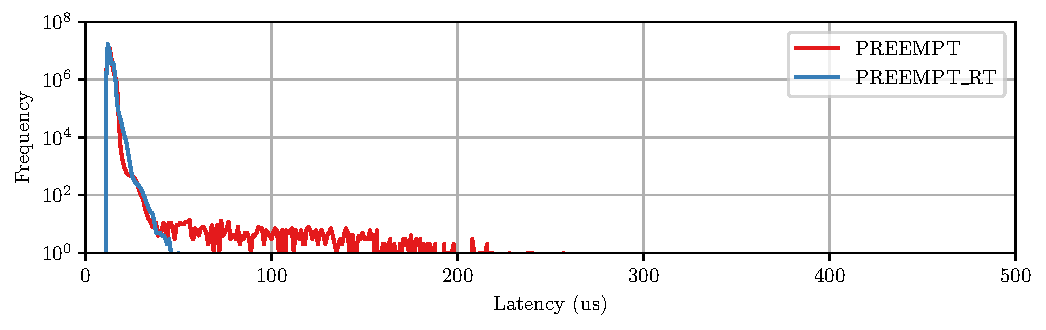
\includegraphics[width=\textwidth]{linux-vs-rt-linux-i100-1h-sc4.pdf}
    \caption[Linux PREEMPT vs PREEMPT\_RT i100 cyclictest results (cpu load)]
    {Linux PREEMPT vs PREEMPT\_RT i100 cyclictest results (cpu load)}
    \label{fig:linux-vs-rt-linux-i100-1h-sc4}
\end{figure}

% MEM LOAD - PREEMPT vs PREEMPT\_RT
\begin{figure}[ht]
    \centering
    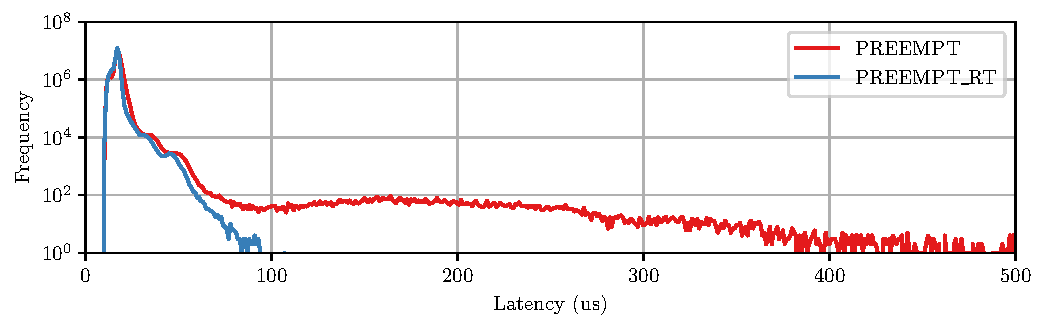
\includegraphics[width=\textwidth]{linux-vs-rt-linux-i100-1h-sm4.pdf}
    \caption[Linux PREEMPT vs PREEMPT\_RT i100 cyclictest results (memory load)]
    {Linux PREEMPT vs PREEMPT\_RT i100 cyclictest results (memory load)}
    \label{fig:linux-vs-rt-linux-i100-1h-sm4}
\end{figure}

\clearpage

\subsubsection{Xen Hypervisor}

After validating the Linux kernel's real-time response, the Xen hypervisor can be evaluated using Linux as both Dom0 and a DomU guest. To ensure that the Xen scheduler itself did not interfere with any results, all vCPUs were assigned on a one to one mapping of real CPUs using the 'null' scheduler. 

As shown in \autoref{fig:xen-rt-slop-i100-1h}, when Xen was evaluated using rt-tests at an interval of $100{\mu}s$ an almost even distribution of latencies is produced. This is very different to what was observed with bare-metal Linux.

\begin{figure}[ht]
    \centering
    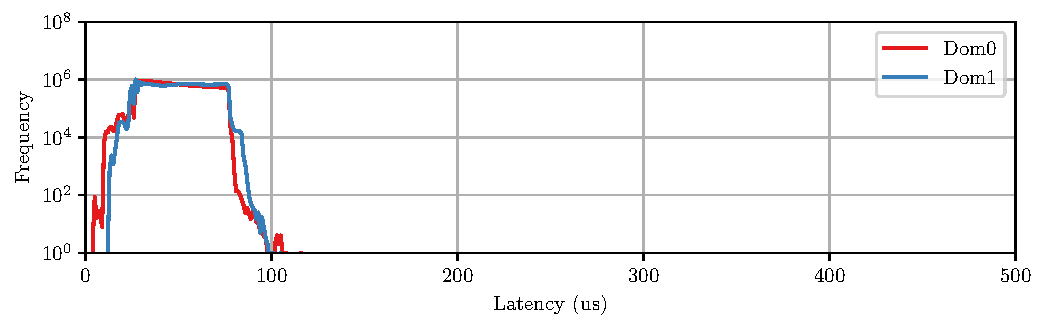
\includegraphics[width=\textwidth]{xen-rt-slop-i100-1h.pdf}
    \caption[Xen i100 cyclictest results (idle)]
    {Xen i100 cyclictest results (idle)}
    \label{fig:xen-rt-slop-i100-1h}
\end{figure}

In attempt to find the cause of the increased latencies, Xen was measured again at a range of intervals ($100{\mu}s$, $200{\mu}s$, $500{\mu}s$ and $1000{\mu}s$) in \autoref{fig:xen-rt-slop-i100-i1000-1h}. The even distribution affect is less noticeable on tests with larger intervals.

\begin{figure}[ht]
    \centering
    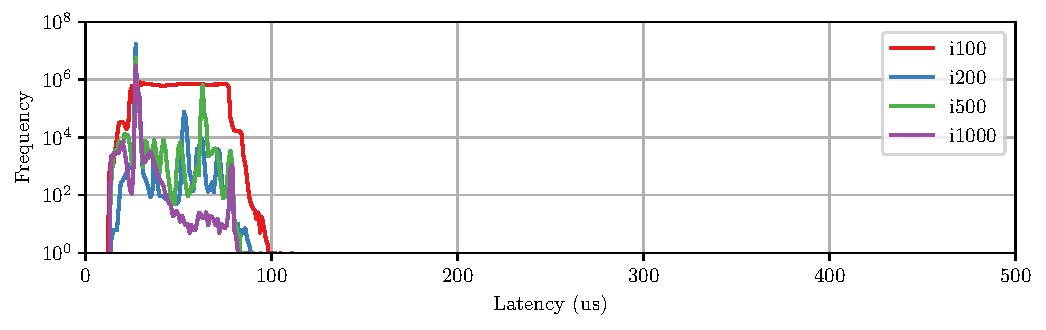
\includegraphics[width=\textwidth]{xen-rt-slop-i100-i1000-1h.pdf}
    \caption[Xen i100, i200, i500, i1000 cyclictest results (idle)]
    {Xen i100, i200, i500, i1000 cyclictest results (idle)}
    \label{fig:xen-rt-slop-i100-i1000-1h}
\end{figure}

This problem has connotations to the issues \textcite{abeniUsingXenKVM2020} experienced with timer resolutions negatively affecting latency evaluations. As cyclictest uses the local CPU timer to measure latencies it is important that it is at a high-enough resolution.

\clearpage

In a PVH virtualisation environment the CPU timers are often virtualized, hence they must be virtualised at high-enough resolution for cyclictest to use. By modifying the \verb|timer_slop| command line property in Xen to $1{\mu}s$ from $50{\mu}s$ the timer resolution was significantly increased. This resulted in much better performance metrics at intervals of $100{\mu}s$ in \autoref{fig:xen-rt-i100-i1000-1h}.

\begin{figure}[ht]
    \centering
    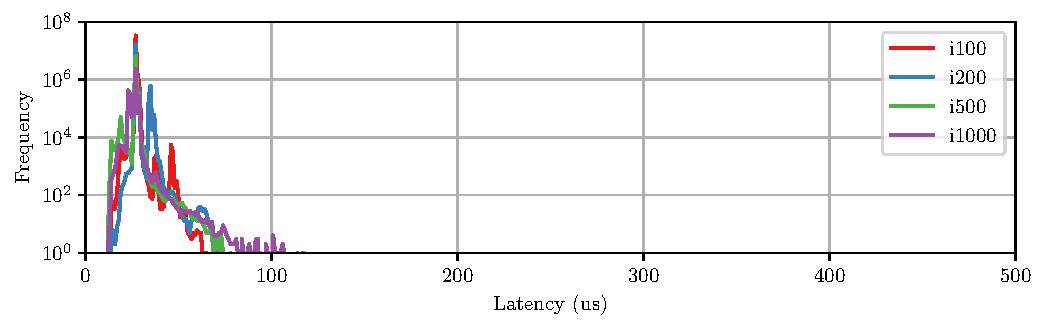
\includegraphics[width=\textwidth]{xen-rt-i100-i1000-1h.pdf}
    \caption[Xen timer adjustment i100, i200, i500, i1000 cyclictest results (idle)]
    {Xen timer adjustment i100, i200, i500, i1000 cyclictest results (idle)}
    \label{fig:xen-rt-i100-i1000-1h}
\end{figure}

To confirm the real-time performance, Xen was also tested with artificial CPU loads in Dom0 and DomU. \autoref{fig:xen-rt-i100-i1000-1h-sc1} shows that there is negligible differences as compared to without load. 

\begin{figure}[ht]
    \centering
    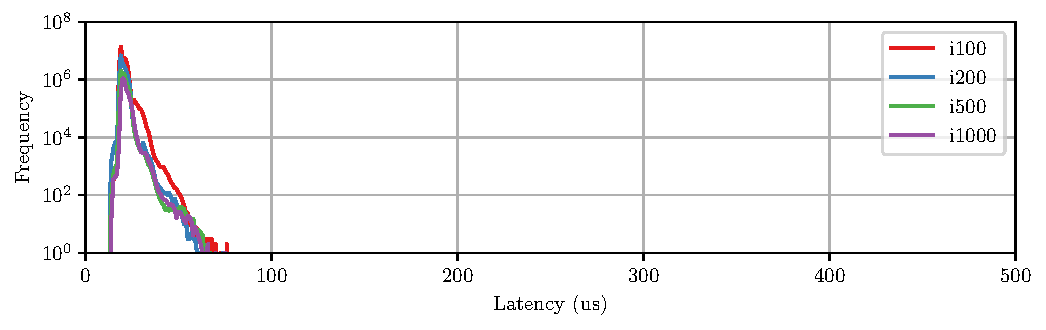
\includegraphics[width=\textwidth]{xen-rt-i100-i1000-1h-sc1.pdf}
    \caption[Xen timer adjustment i100, i200, i500, i1000 cyclictest results (cpu load)]
    {Xen timer adjustment i100, i200, i500, i1000 cyclictest results (cpu load)}
    \label{fig:xen-rt-i100-i1000-1h-sc1}
\end{figure}


\textbf{Evaluation}

Xen approximately doubled the interrupt latency measured as compared to bare-metal Linux. This is not ideal, but Xen could still be used in a soft real-time application if the latencies were accounted for. Before deploying Xen in a real-time environment, additional tests should evaluate the multi-core interference across multiple guest virtual machines.

\clearpage
\graphicspath{{main/design/software/graphics/}}

\subsection{Language}



\clearpage
\graphicspath{{main/design/scheduler/graphics/}}

\section{Scheduler}

To implement an event based scheduler, the scheduler must be able to send signals between processes without significant jitter and latency. This is because the signals effectively send execution requests for each component and if there are significant delays, the component will not execute when desired. The level of latency and jitter that is acceptable can be estimated by calculating a worst case execution time for a control loop in a particular application.

There are several different methods that can be used to send signals between processes in a Linux system. Shared memory, sockets and signalling shall all be investigated as they can be easily migrated onto a non-linux POSIX compatible system if required. This evaluation will focus on gathering latency and jitter metrics for the different techniques.

\subsubsection*{Test Program Design}

Each evaluation will use a parent-child arrangement of processes, whereby a parent process spawns a child processes. These processes will both be given the highest real-time scheduler priority and pinned to two separate cores that are isolated from the operating system. The parent process shall run at a controlled frequency of 100Hz for 10,000 iterations, each iteration will request the child process to execute. At each execution, the time requested $t_0$ and actual execution time $t_1$ shall be recorded, shown in \autoref{fig:parentChildExecuteDelay}. These shall be later evaluated where $\Delta{}t$ is calculated.

% diagram here of the time delay between execution
\begin{figure}[ht]
    \centering
    \begin{sequencediagram}
        \newthread{p}{Parent}
        \newthreadShift{c}{Child}{4cm}

        \mess[1]{p}{}{c}
        \node[anchor=east] (t0) at (mess from) {$t_0$};
        \node[anchor=west] (t1) at (mess to) {$t_1$};

        \path (t0.east) |- coordinate(t12) (t1); \draw[dashed] (t1) -- (t12);
        \node[anchor=south west] at (t12) {$\Delta{}t$};

    \end{sequencediagram}
    \caption{Parent-child process execution delay}
    \label{fig:parentChildExecuteDelay}
\end{figure}


% diagram of the time delay

\subsubsection*{Implementation}

Test programs will execute on the target development hardware (CM4) with Linux kernel 6.1.65 and the real-time kernel batch applied. These programs will use the Rust programming language, this is to align with the final development software infrastructure. To set schedule parameters and interface with Linux they shall use the \verb|libc| crate \autocite{RustlangLibc2024}. In addition, they will use the \verb|csv| crate \autocite{gallantBurntSushiRustcsv2024} to save timing data to a csv file.

\newpage

\subsection{Shared Memory}

% present tense
On a UNIX system each process has its own virtual memory space, so no process can normally access the memory of another process. This is to ensure isolation between processes. Shared memory can be used to allow multiple processes to access the same memory segment, though synchronisation methods such as mutexes must be used to ensure data and program integrity. \autocite{SharedMemory}

To allocate \verb|shmget()| returns an identifier \verb|shm_id| that can later be used to access the memory segment. \autocite{ShmgetLinuxManual}. To add the memory segment to the current processes the \verb|shmat()| function is used, when provided with the \verb|shm_id| \autocite{ShmopLinuxManual}.

To access the shared memory functionality of Linux in the Rust language this test will use the \verb|shared_memory| crate  \autocite{elast0nyElast0nyShared_memory2024}. The parent process shall create two shared memory locations and a files containing the \verb|shm_id|. Using the shared memory, event synchronisation data structures can be created using the \verb|raw_sync| crate \autocite{elast0nyElast0nyRaw_syncrs2024}. These events can then be used to signal when the child process should execute \verb|send_event| and its completion \verb|recv_event|. Next, the parent shall spawn the child process which will indefinitely loop and wait (blocked) for an event to execute.

\begin{figure}[ht]
    \centering
    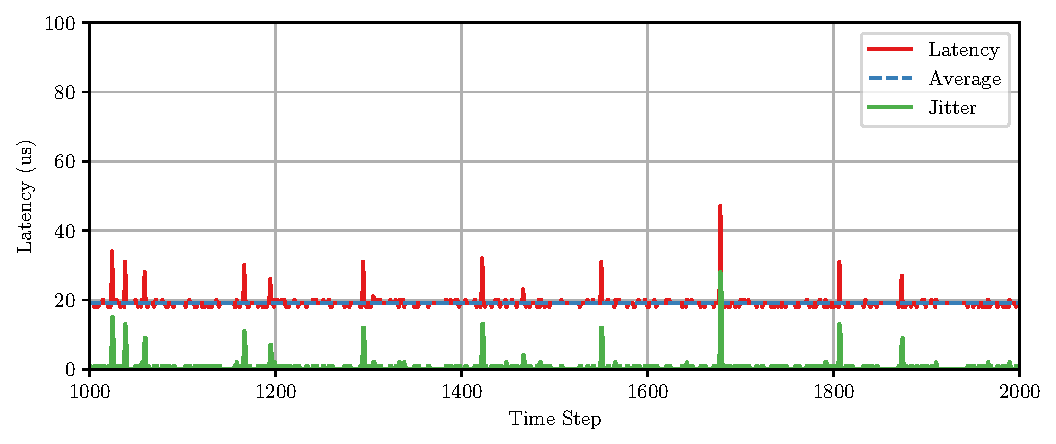
\includegraphics[width=\textwidth]{rt-pi4-mem-times.pdf}
    \caption[Experiment latency graph for shared memory]
    {Experiment latency graph for shared memory}
    \label{fig:rtPi4MemTimes}
\end{figure}

The 

\newpage

\subsection{Sockets}

% present tense
Unix sockets explain

% past tense

\begin{figure}[ht]
    \centering
    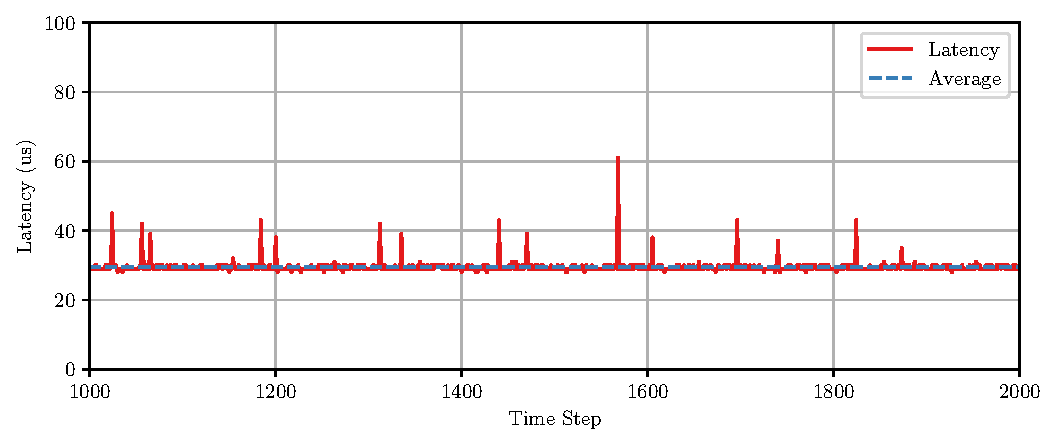
\includegraphics[width=\textwidth]{rt-pi4-socket-times-blocking.pdf}
    \caption[Experiment latency graph for blocking sockets]
    {Experiment latency graph for blocking sockets}
    \label{fig:rtPi4SocketTimesBlocking}
\end{figure}

Although the blocking socket test did perform reasonably well, it was on average over 50\% slower than the shared memory implementation.

\begin{figure}[ht]
    \centering
    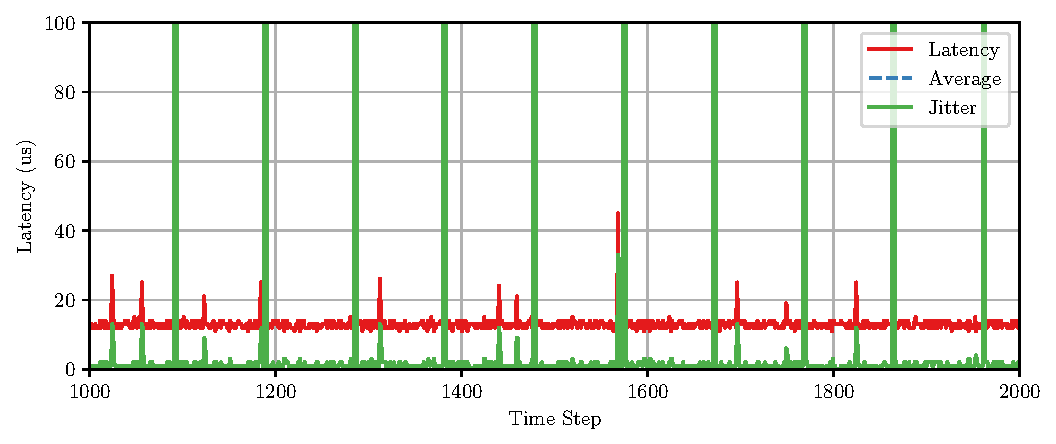
\includegraphics[width=\textwidth]{rt-pi4-socket-times.pdf}
    \caption[Experiment latency graph for non-blocking sockets]
    {Experiment latency graph for non-blocking sockets}
    \label{fig:rtPi4SocketTimes}
\end{figure}

The non-blocking socket performed much better than both the blocking socket and events in shared memory. However, approximately 100 cycles (1 second) significant latencies were introduced at over 40ms, making this solution unviable for a real-time system. It is assumed that these latencies are introduced periodically due to the kernel itself being moved onto the CPU. As the program is busy waiting it never enters the blocked state. Therefore it consumes 100\% of the CPU resources with no opportunity for the kernel to perform management functions.

One possible implementation for the scheduler could use a combination of both the blocking and non blocking sockets. The scheduler could first wakeup a component process using a blocking socket, once on the processor the component can now busy wait for a short period of time on the non blocking socket. Then the scheduler can send the execute command. This reduces the uncertainty of when the process will execute, but overall takes much longer to execute a component as two sequential messages are sent.

To work around this the components could be put into the busy state on alternating processors. So component $a$ could be put into the busy wait and executed, while component $b$ is in the blocked state. These could then be alternated. While this would improve the real-time response of the system, it would unnecessarily consume CPU resources.

\newpage

\subsection{Signalling}

\begin{figure}[ht]
    \centering
    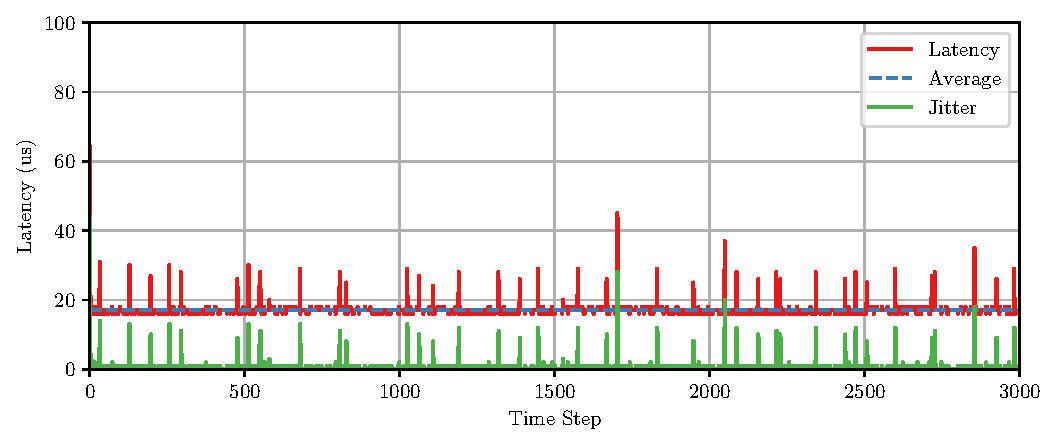
\includegraphics[width=\textwidth]{rt-pi4-signal-times.pdf}
    \caption[Experiment latency graph for signals]
    {Experiment latency graph for signals}
    \label{fig:rtPi4SignalTimes}
\end{figure}

\newpage

\subsection{Evaluation}

\begin{figure}[ht]
    \centering
    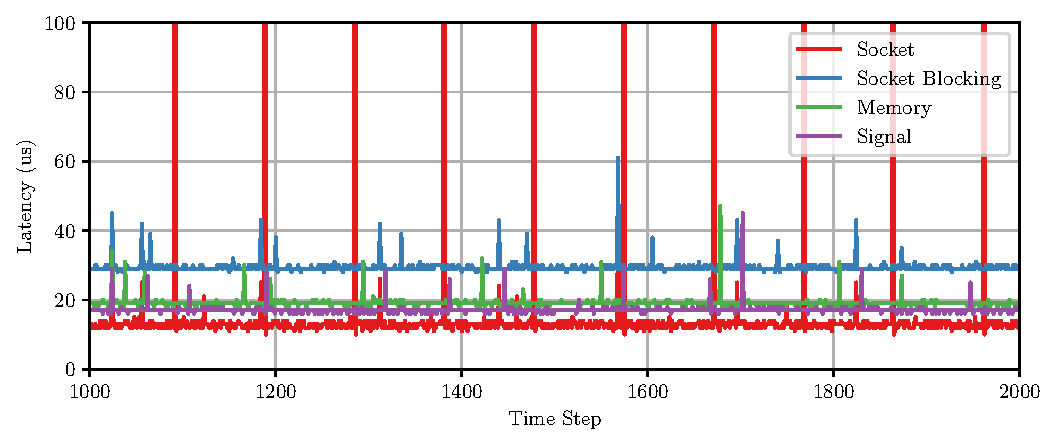
\includegraphics[width=\textwidth]{rt-pi4-compare-times.pdf}
    \caption[Comparison experiment latency graph for all methods]
    {Comparison experiment latency graph for all methods}
    \label{fig:rtPi4CompareTimes}
\end{figure}

\begin{figure}[ht]
    \centering
    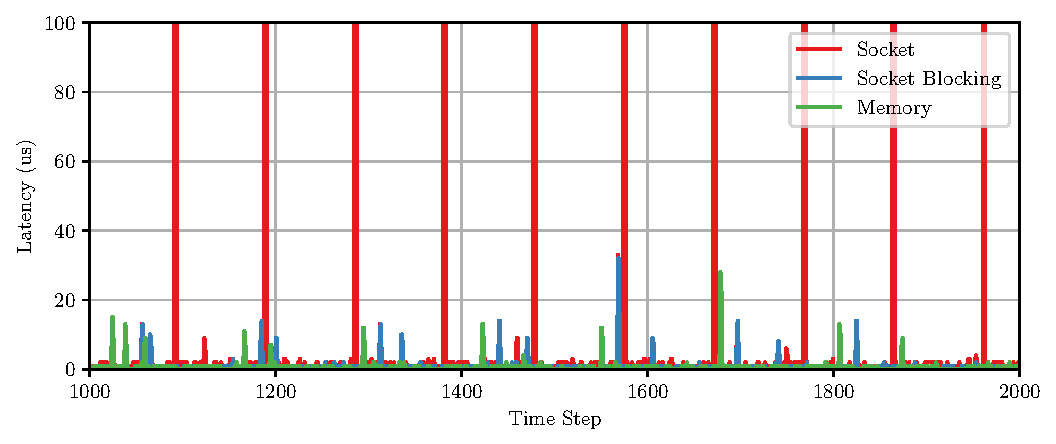
\includegraphics[width=\textwidth]{rt-pi4-compare-times-jitter.pdf}
    \caption[Comparison experiment latency graph for all methods]
    {Comparison experiment jitter graph for all methods}
    \label{fig:rtPi4CompareTimesJitter}
\end{figure}

\subsubsection*{Processor Differences}

% Mention something to do with the Raspberry Pi 5 vs 4 

\begin{figure}[ht]
    \centering
    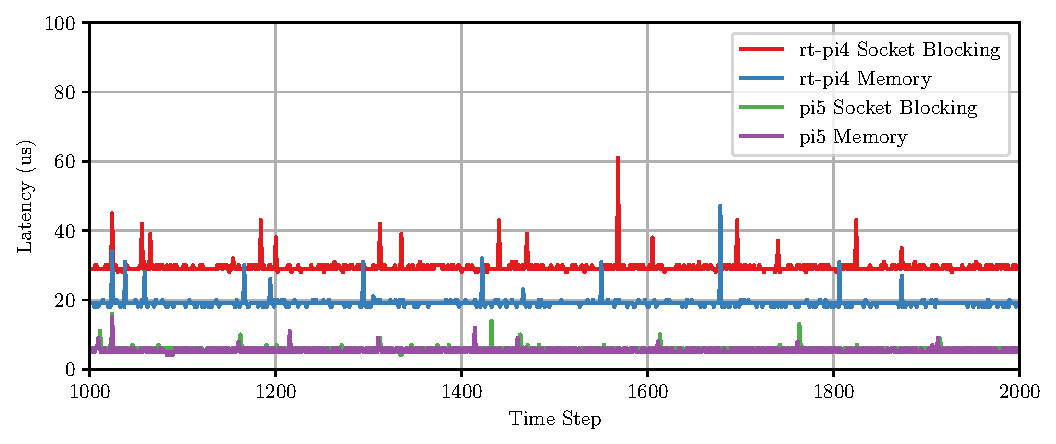
\includegraphics[width=\textwidth]{rt-pi4-vs-pi5.pdf}
    \caption[Comparison experiment latency graph for all methods on Raspberry Pi 4 vs 5]
    {Comparison experiment latency graph for all methods on Raspberry Pi 4 vs 5}
    \label{fig:rtPi4vsPi5CompareTimes}
\end{figure}

\begin{figure}[ht]
    \centering
    \begin{sequencediagram}
        \newinst{r}{Runner}
        \newinst[6]{c}{Component}

        \mess[1]{r}{Execute}{c}
        \mess[1]{c}{Acknowledge}{r}
        \mess{r}{Wake}{c}
        \mess{c}{Acknowledge}{r}

        \stepcounter{seqlevel}

        \mess[1]{r}{Execute}{c}
        \mess[1]{c}{Acknowledge}{r}
        \mess{r}{Wake}{c}
        \mess{c}{Acknowledge}{r}

    \end{sequencediagram}
    \caption{Client-Server messaging}
\end{figure}

\clearpage
\section{Software}

% \section{Operation}

% \begin{sequencediagram}
%     \newthread[white]{c}{CLI}
%     \newinst[3]{a}{Agent}
%     \newinst[3]{r}{Runner}

%     \begin{call}{c}{Init()}{a}{}
%     \end{call}
% \end{sequencediagram}

% \begin{tikzpicture}
%     \begin{package} {State} 
%         \begin{class}[text width=8cm]{StateManager} {0,0}
%             \attribute{stream : UnixStream}
%             \attribute{data : Vecu8}
%             \operation{new(UnixStream) : self}
%             \operation{run}
%             \operation{getdata : Vecu8}
%             \operation{setdata(Vecu8) : Done}
%         \end{class}

%         \begin{class}[text width=8cm]{CommunicationManager} {-5,-5}
%             \attribute{stream : UnixStream}
%             \attribute{data : Vecu8}
%             \operation{new(UnixStream)}
%             \operation{run}
%             \operation{getdata : Vecu8}
%             \operation{setdata(Vecu8) : Done}
%         \end{class}
%     \end{package}

%     % \begin{class}[text width=8cm]{ClassName}{0,0}
%     %     \attribute{name : attribute type}
%     %     \attribute{name : attribute type = default value}
%     %     \operation{name(parameter list) : type of value returned}
%     %     \operation[0]{name(parameters list) : type of value returned}
%     % \end{class}
% \end{tikzpicture}

% \tikzset{
%     ->,
%     >=stealth,
%     node distance=3cm,
%     every state/.style={thick, fill=gray!10},
%     initial text=$ $,
% }

% \begin{tikzpicture} 
%     \node[state, initial, accepting] (1) {$1$};
%     \node[state, below left of=1] (2) {$2$};
%     \node[state, right of=2] (3) {$3$};
%     \draw   (1) edge[above] node{$b$} (2)
%                 (1) edge[below, bend right, left=0.3] node{$\epsilon$} (3)
%                 (2) edge[loop left] node{$a$} (2)
%                 (2) edge[below] node{$a, b$} (3)
%                 (3) edge[above, bend right, right=0.3] node{$a$} (1);
% \end{tikzpicture}

% why rust ferrocene, ada

% \begin{itemize}
%     \item Create Component \textbf{Non-Blocking}
%     \begin{itemize}
%         \item Component Identifier
%     \end{itemize}
%     \item Start Component \textbf{Blocking}
%     \begin{itemize}
%         \item Component Identifier
%     \end{itemize}

%     \item Stop Component \textbf{Blocking}
%     \begin{itemize}
%         \item Component Identifier
%     \end{itemize}

%     \item Remove Component \textbf{Non-Blocking}
%     \begin{itemize}
%         \item Component Identifier
%     \end{itemize}
    
%     \item Add Route \textbf{Blocking}
%     \begin{itemize}
%         \item Component Identifier
%     \end{itemize}

%     \item Remove Route \textbf{Blocking}
%     \begin{itemize}
%         \item Component Identifier
%     \end{itemize}

%     \item Set Schedule \textbf{Blocking}
%     \begin{itemize}
%         \item Component Identifier
%     \end{itemize}

%     \item Add State Synchronisation \textbf{Blocking}
%     \begin{itemize}
%         \item Component Identifier
%     \end{itemize}

%     \item Remove State Synchronisation \textbf{Blocking}
%     \begin{itemize}
%         \item Component Identifier
%     \end{itemize}
    
%   \end{itemize}


% middleware
    % message passing
    % scheduler
    % state sync
    % configuration
        % background thread
        % state machines
